\documentclass[../Main/main.tex]{subfiles}

\begin{document}
	\graphicspath{{../Discretization/figs/}}
	\chapter{Numerical approximation techniques}
	\section{The Finite Element Method}
	\addcontentsline{toc}{section}{Finite Element Method}
	The finite element method was first developed in the 1940s by Richard Courant for problems in solid mechanics. As computers became better in the 1960s the method became  more mainstream \cite{Stein2014}. Today there are several general purpose finite element programs being used for a wide range of problems.\par
	In this chapter we will introduce the finite element method and state results about stability and convergence.
	We will concentrate on solving the Poisson equation. Let $\Omega \subset \mathbb{R}^n$ be some open and bounded domain. Find $u$ such that:
	\begin{equation} \label{eq:poisson}
		\begin{split}
			-\nabla \cdot \bm{K} \nabla u(x) &= f(x) \ \  x\in \Omega \\ 
			u(x) &= 0 \ \ x\in \partial \Omega.
		\end{split}
	\end{equation}
	For this equation to be well defined we require that $u$ has double derivatives in $\Omega$, but it is easy to come across physical examples where this does not make sense.
	This is some of the motivation for formulating the Poisson equation in the \emph{variational formulation}. Another motivation is that it allows for an nice framework for computing the solution, as we will soon see. But first, we study some spaces of functions and their properties.
	
	
	\subsection{Function spaces}
	\addcontentsline{toc}{subsection}{Function spaces}
	When discussing PDE's and the numerical schemes to solve them it is important to have a precise notion of what kind of functions we are looking for and their properties. The function spaces discussed here are all normed vector spaces. From now on we assume that $\Omega \subset \mathbb{R}^d$ is a bounded domain.
	\begin{definition}[Lebesgue spaces, $L^p(\Omega)$]
		For $p\in [1,\infty)$ let $L^p(\Omega)$ be the space of functions for which  $\left \| u \right \|_p = (\int_{\Omega} u^pdx)^{1/p} <\infty$
	\end{definition}

	\begin{remark}
		Note that an $L^p(\Omega)$ norm induces equivalence relations on the set of functions. Two functions in $L^p(\Omega)$ are equal if they only differ on a set of measure zero.
	\end{remark}
	An important concept when discussing normed vector spaces are that they intuitively do not have any points missing, this is formally defined as spaces where every Cauchy sequence converges. This is known as \emph{complete} vector spaces or \emph{Banach spaces}.
	
	\begin{theorem}[Riesz-Fischer Theorem \cite{Cheney} chapter 8]\label{theorem:Riesz-Fischer}
		Each $L^p(\Omega)$ space is a Banach space.
	\end{theorem}
	\begin{remark}
		The space $L^2(\Omega)$ is a inner product space, with inner product
		\begin{equation*}
			\left \langle u,v\right \rangle_{L^2} = \int_{\Omega}uv \ dx.
		\end{equation*}
		 Banach spaces with an inner product, that induces the norm 
		\begin{equation*}
			\left \langle u,u \right \rangle ^{\frac{1}{2}} = \left \| u \right \|,
		\end{equation*}
		are called \textbf{Hilbert spaces}. 
	\end{remark}
	
	
	
	
	Before we continue the study of function spaces we develop some convenient notation for derivatives.
	
	\begin{definition}[multi-index notation]
		Let $\overline{\alpha}$ be an ordered n-tuple. We call this a multi-index and denote the length $|\overline{\alpha}| = \sum_{i=1}^n 		\alpha_i$.
		For $\phi \in C^{\infty}(\Omega)$ we define $D^{\overline{\alpha}} = (\frac{\partial }{\partial x_1})^{\alpha_1}(\frac{\partial }{\partial x_2})^{\alpha_2}...(\frac{\partial }{\partial x_n})^{\alpha_n}\phi$
	\end{definition}
	
	We would also like a more general notion of derivative than the one presented in A basic calculus book.
	\begin{definition}[weak derivative]
		Let $L_{loc}^1(\Omega) =\left \{  \right. f\in L^1(K):\forall K \in \Omega \text{  where K is compact}\left.  \right \}$.
		Let $f \in L_{loc}^1(\Omega)$. If there exists $g\in L_{loc}^1 (\Omega)$ such that 
		\begin{equation}
			\int_{\Omega} g \phi dx = (-1)^{|\overline{\alpha}|} \int_{\Omega} f D^{\overline{\alpha}} \phi dx \ \ \forall \phi \in C^{\infty}
		\end{equation}
		 with $\phi = 0$ on $\partial \Omega$  we say that $g$ is the weak derivative of $f$ and denote it by $D_w^{\overline{\alpha}}f$.
	\end{definition}
	
	
	We can now define a class of subspaces of the $L^p$ spaces known as the \textbf{Sobolev spaces}
	\begin{definition}[Sobolev space]
		Let $k$ be a non-negative integer, define the Sobolev norm as 
		\begin{equation*}
			\left \| u \right \|_{W^{k,p}(\Omega)} := \left (\sum_{|\overline{\alpha}| \leq k} \left \| D_w^{\overline{\alpha}}u \right \|_{L^p(\Omega)}^p\right )^{1/p}.
		\end{equation*}
		We then define the sovolev spaces as 
		\begin{equation*}
			W^{k,p}(\Omega) = \left \{  \right. f\in L^1_{loc}(\Omega):\left \| f \right \|_{W^{k,p}}<\infty \left.  \right \}.
		\end{equation*}
	\end{definition}
	\begin{theorem}
		The Sobolev spaces $W^{k,p}(\Omega)$ are Banach spaces
	\end{theorem}
	
	\begin{proof}
		Let $\left \{  u_i\right \}_{i=0}^{\infty} \subseteq W^{k,p}(\Omega)$ be a Cauchy sequence. This implies that for all $\overline{\alpha}, \  |\overline{\alpha}| \leq k$ we have a Cauchy sequence in $L^p(\Omega)$:
		\begin{gather*}
			\left \| u_j -u_i \right \|_{W^{k,p}} =
			(\sum_{|\overline{\alpha}|\leq k} \left \| D_w^{\overline{\alpha}}u_j - D_w^{\overline{\alpha}}u_i \right \|_{L^p(\Omega)}^p)^{1/p}  < \epsilon \ \forall i,j \geq N \\
			\implies \left \| D_w^{\overline{\alpha}}u_j - D_w^{\overline{\alpha}}u_i \right \|_{L^p(\Omega)} < \epsilon
		\end{gather*}
		By \eqref{theorem:Riesz-Fischer}, every $L^P(\Omega)$ space is a Banach space. Therefore, for each $|\overline{\alpha}| \leq k$, $D_w^{\overline{\alpha}}u_i $ converges to some limit, $ u_{\overline{\alpha}}\in L^p(\Omega)$, as $i\rightarrow  \infty$. In particular $u_i \rightarrow u$ in  $L^p(\Omega)$, so the limit in the $\left \|\cdot \right \|_{W^{k,p}(\Omega)}$ norm, $u$, is well defined. Now we need to show that $\left \{ u_{\overline{\alpha}} \right \}_{\overline{\alpha}}$, are in fact the weak derivatives of $u$, ie. $D_w^{\overline{\alpha}}u =  u_{\overline{\alpha}}$. In other words, that the limit of $u_i$ in the $\left \|\cdot \right \|_{W^{k,p}(\Omega)}$ norm, $u$, is in fact in $W^{k,p}(\Omega)$. By the definition of weak derivative we have:
		\begin{gather*}
			\int_{\Omega} D_w^{\overline{\alpha}}u_i \phi dx = (-1)^{|\overline{\alpha}|} \int_{\Omega} u_i D^{\overline{\alpha}}\phi dx
		\end{gather*}
		Let $1=\frac{1}{q}+\frac{1}{p}$, applying Hölder's inequality on both sides we get the two inequalities:
		\begin{gather*}
			\int_{\Omega} (D_w^{\overline{\alpha}}u_i - u_{\overline{\alpha}}) \phi dx \leq \left \| D_w^{\overline{\alpha}}u_i - u_{\overline{\alpha}} \right \|_{L_p} \left \| \phi \right \|_{L_q} \\
			\int_{\Omega} (u_i -u) D^{\overline{\alpha}}\phi dx \leq \left \|u_i -u  \right \|_{L_p} \left \| D^{\overline{\alpha}}\phi \right \|_{L_q}
		\end{gather*}
		Taking the limit, the right hand side goes to zero, and we end up with the fact that we can move the limit out of the integral:
		\begin{gather*}
			\lim_{i\rightarrow \infty} \int_{\Omega} D_w^{\overline{\alpha}}u_i \phi dx =  \int_{\Omega}u_{\overline{\alpha}} \phi dx \\
			\lim_{i\rightarrow \infty}\int_{\Omega} u_i D^{\overline{\alpha}}\phi dx = \int_{\Omega} u  D^{\overline{\alpha}}\phi dx
		\end{gather*}
		Now we can put the two equations together with the definition of the weak derivative:
		\begin{equation*}
			\int_{\Omega}u_{\overline{\alpha}} \phi dx = \lim_{i\rightarrow \infty} \int_{\Omega} D_w^{\overline{\alpha}}u_i \phi dx = \lim_{i\rightarrow \infty}(-1)^{|\overline{\alpha}|}\int_{\Omega} u_i D^{\overline{\alpha}}\phi dx = \int_{\Omega} u  D^{\overline{\alpha}}\phi dx.
		\end{equation*}
		We have shown $D_w^{\overline{\alpha}}u =  u_{\overline{\alpha}}$, and therefore, that $u\in W^{k,p}(\Omega)$. 
	\end{proof}
	\begin{definition}
		We rename the $L^2(\Omega)$ based Sobolev spaces as follows 
		\begin{equation*}
			H^k(\Omega) = W^{k,2}(\Omega)
		\end{equation*}
		With the norm of $H^k(\Omega)$ being written in the more compact form $\left \| \cdot \right \|_k$ and the inner product defined as follows:
		\begin{equation*}
			\left \langle u,v \right \rangle_k = \sum_{|\overline{\alpha}| \leq k} \int_{\Omega}D_w^{\overline{\alpha}}u,D_w^{\overline{\alpha}}v dx.
		\end{equation*}
	\end{definition}

	In Sobolev spaces it is not obvious that a function is well defined on a lower dimensional subset of $\Omega$, because two functions may map elements of this zero measure subset to different values and still be of the same equivalence class. This is important to settle if we want to solve boundary value problems. The following results holds for general $L^p(\Omega)$ based Sobolev spaces, but we will only state them for the Hilbert space $H^1(\Omega)$.
	\begin{definition}
		We denote by $H_0^{k}(\Omega)$ the closure of $C_c^{\infty}(\Omega)$ in $H^{k}(\Omega)$, where $C_c^{\infty}(\Omega)$ is the space of infinitely differentiable functions with compact support.
	\end{definition}
	\begin{theorem}[Trace theorem, (Evans \cite{evans10}, chapter 5)]
		Assume $U$ is bounded and $\partial U$ is $C^1$. Then there exists a bounded, linear operator
		\begin{equation*}
			T: H^{1}(U) \rightarrow L^2(\partial U)
		\end{equation*}
		Such that
		\begin{enumerate}
			\item $ Tu = u|_{\partial u} $ if $u\in H^{1}\cap C(\overline{U})$
			\item $\left \|Tu\right\|_{L^p(\partial U)}\leq \left \| u \right \|_{H^{1}(U)}$
		\end{enumerate}
	\end{theorem}
	We call $Tu$ the trace of $u$. Note that the theorem does not state that $T$ is surjective.
	\begin{theorem}(Trace-zero functions in $W^{1,p}$,(Evans \cite{evans10}, chapter 5))
		Suppose $U$ is as in the previous theorem and $u\in W^{1,p}(U)$, then
		\begin{equation*}
			u\in H^{1}_0 \Leftrightarrow  Tu=0 \textit{ on }\partial U
		\end{equation*}
	\end{theorem}
	
	\begin{remark}
		We often denote the image of $T$ as:
		\begin{equation*}
			 H^{\frac{1}{2}}(\Omega) = T(H^1(\Omega))
		\end{equation*}
		And define the norm
		\begin{equation*}
			\left \|f\right \|_{H^{\frac{1}{2}}(\Omega)} = \inf_{w\in H^1(\Omega), \ Tw=f} \left \| w \right \|_1
		\end{equation*}
	\end{remark}
	Now we have the theory we need to study elliptic boundary value problems and their weak solutions.
	\subsection{The variational problem}
	\addcontentsline{toc}{subsection}{The variational problem}
	We obtain the \textbf{variational formulation} of \eqref{eq:poisson} with multiplying \eqref{eq:poisson} by a function $v$ in a suitable space $V$ called the \emph{test space}, integrating over $\Omega$ and using integration by parts/divergence theorem.
	\begin{equation*}
		-\int_{\Omega}v\nabla \cdot\bm{K}\nabla u \ dx = -\int_{\partial \Omega}v \bm{K}\nabla u \cdot \bm{n} \ dx + \int_{\Omega}(\nabla v)^{T}\bm{K} \nabla u \ dx = \int_{\Omega}vf\ dx
	\end{equation*}
	If we choose $v$ such that $v=0$ on $\partial \Omega$, then the integral over the boundary vanishes. The new formulation reads: find $u$ such that 
	\begin{equation}\label{eq:variational poisson}
			 \int_{\Omega}(\nabla v)^T \bm{K} \nabla u \ dx = \int_{\Omega}vf\ dx \ \ \  \forall v \in V.
	\end{equation}
	A good choice of the test space $V$ is $V=H_0^1(\Omega)$. We also choose this as the solution space.
	We see that if $u$ is a solution to \eqref{eq:poisson}, it also solves \eqref{eq:variational poisson}. But a solution to \eqref{eq:variational poisson} does not necessarily solve \eqref{eq:poisson}, that is why it is also called the \emph{weak formulation}.\par
	The variational problems that we will look at, will all have the form: Find $u$ such that
	\begin{equation}\label{eq:variational problem}
			a(u,v) = b(v) \ \ \ \forall v \in V,
	\end{equation}
	where $a(\cdot,\cdot)$ is a \emph{bilinear form} on $V$ and $b(\cdot)$ is a \emph{linear functional} on $V$. To be precise we define a famous concept from functional analysis:
	\begin{definition}[dual space]
		Let $V$ be a normed vector space, then we define it's dual space as the space of functions from $V$ to $\mathbb{R}$ that are linear and continuous, also called linear functionals. We denote it by $V^{'}$. This is a normed vector space with the norm: \begin{equation*}
\left \| v \right \|_{V'} = \sup \left \{ |\phi(u)|:\left \| u\right \|_V = 1 \right \}. 		\end{equation*}
	\end{definition}
	In general, a variational formulation can we seen as finding the element in a Banach space that is mapped to an element in its dual space by some map.
	\subsubsection*{Boundary conditions}
	Let $\partial \Omega = \Gamma_D\bigcup \Gamma_N$ with $\Gamma_D \bigcap \Gamma_N = \emptyset$, then \eqref{eq:poisson} with more complicated boundary conditions can be written:
	\begin{equation}\label{eq:inhomogenous poisson}
		\begin{aligned}[c]
			 - \nabla \cdot \bm{K} \nabla \hat{u}(x) &= f(x) \\
			\hat{u}(x) &= g_D \\
			\bm{K}\nabla \hat{u}(x) &= g_N
		\end{aligned}
		\ \ \
		\begin{aligned}[c]
			x &\in \Omega  \\
			x &\in \Gamma_D \\
			x &\in \Gamma_N
		\end{aligned}
	\end{equation}
	To make a variational formulation of \eqref{eq:inhomogenous poisson} we first define the test space:
	\begin{equation*}
		V = \left \{ v\in H^1(\Omega): T(v)=0 \text{ on }\Gamma_D\right \}
	\end{equation*}
	Next, we define the bilinear form:
	\begin{equation}
		a(u,v) := \int_{\Omega} \nabla u \bm{K} \nabla v \ dx.
	\end{equation}
	Further, assume there exists an element $w$ of $ H^1(\Omega)$ that are mapped by the trace operator such that Dirichlet boundary conditions are met: $T(w)=g_D$. Let $\hat{u} = u+w$, now we can use integration by parts to as before:
	\begin{equation}
		a(u+w,v) = \int_{\Omega}(\nabla u+\nabla w)^{T}\bm{K} \nabla v \ dx = \int_{\Omega}fv \ dx -\int_{\partial\Omega}\bm{K}\nabla (u+w)\cdot \bm{n}v \ dx .
	\end{equation}
	Using the linearity of $a(\cdot,\cdot)$ and inserting boundary conditions we get:
	\begin{equation}\label{eq:inhomogenous poisson weak}
		a(u,v) = b(v)= \int_{\Omega} fv \ dx - \int_{\Omega}(\nabla w)^T\bm{K} \nabla v \ dx - \int_{\Gamma_N} g_N v \ dx.
	\end{equation}
	Hence both Dirichlet and Neumann boundary conditions are incorporated into the right hand side. For homogeneous Dirichlet boundary conditions, the second term on the right hand side of \eqref{eq:inhomogenous poisson weak} vanishes. 
	
	\subsection{Existence and uniqueness}
	\addcontentsline{toc}{subsection}{Existence and uniqueness}
	We still need to show that \eqref{eq:inhomogenous poisson weak} has an unique solution.
	First we define some important properties that a variational problem should have in order to have a unique solution. Let $(V,\left \| \cdot \right \|_V)$ be a Hilbert space.
	\begin{definition} Let $a(\cdot,\cdot):V\times V \rightarrow \mathbb{R}$ be a \emph{bi linear form}. We say that:
			\begin{itemize}
			\item $a(\cdot,\cdot)$ is \textbf{coercive with respect to }$V$, or \textbf{elliptic} if there exists a constant $C_c\in \mathbb{R}$ such that $C_c\left \| u \right \|_V^2 \leq a(u,u) \ \forall u \in V$
			\item $a(\cdot,\cdot)$ is \textbf{bounded} or \textbf{continuous} if there exists a constant $C_B$ such that $|a(u,v)|\leq C_B\left \| u \right \|_V\left \| v \right \|_V \ \forall u,v \in V$
			\end{itemize}
	\end{definition}
	To use this to prove existence and uniqueness, we must first state some important results about the underlying space $V$. The following theory can be found in it's entirety in chapter one-four of Cheney \cite{Cheney}
	\begin{theorem}\label{th:decomposition of hilbert}
		If $Y$ is a closed subspace of a Hilbert space $X$, then $X = Y\otimes Y^{\bot}$ \\
		Where $Y^{\bot} = \left \{ \left. x\in X: \left \langle x,y \right \rangle=0 \ \forall y \in Y \right \} \right.$ is orthogonal complement.\\ That is: an element in $X$ can always be written as the sum of an element $Y$ and an element in $Y^{\bot}$.
	\end{theorem}
	\begin{theorem}[Riesz representation theorem]\label{th:riesz representation}
		Every continuous linear functional defined on a Hilbert space $X$ can be written $x\rightarrow \left \langle x,v \right \rangle$ for a uniquely determined $v \in X$.
	\end{theorem}
	\begin{proof}
		Let $\phi \in X'$, define $Y = \left \{ x\in X:\phi (x)=0 \right \}$ to be the null space of $\phi$. Take a non-zero vector in the orthogonal complement $u\in Y^{\bot}$ such that $\phi (u)=1$, (if this does not exist then $X=Y$ and $\phi (x) = \left \langle x, 0\right \rangle$, this is ensured by theorem \ref{th:decomposition of hilbert}). Now we can write every vector in $X$ as a linear combination of a vector in $Y$ and the vector $u$. $x = x-\phi (x) u + \phi(x) u$ for any $x \in X$. Using this, we can find an expression for the inner product of $x$ with a scaled version of $u$ \\
		$\left \langle x,\frac{u}{\left \| u \right \|^2} \right \rangle  = \left \langle x-\phi (x)u,\frac{u}{\left \| u \right \|^2} \right \rangle + \left \langle \phi (x)u,\frac{u}{\left \| u \right \|^2} \right \rangle $.
		The first part of the sum vanishes as $x - \phi (u)x \in Y$. So we end up with \\
		$\left \langle x,\frac{u}{\left \| u \right \|} \right \rangle  = \phi (x)\frac{\left \langle u,u\right \rangle}{\left \| u \right \|^2} = \phi (x)$ \\
	\end{proof}
	\begin{theorem}[Banach fixed point theorem]\label{th:Banach}
		Let $X$ be a Banach space and $F:X\rightarrow X$ an operator where $\left \|Fx-Fy\right \|_X\leq \theta \left \| x-y \right\|_X$ for some $\theta \in (0,1)$, we call this a \textbf{contraction}.\\
		Then for all $x \in X$ the sequence $[x,Fx,F^2x,...]$ converges to a point $x^* \in X$ called the fixed point of $F$.
	\end{theorem}
	See page 177 of \cite{Cheney} for a proof.
	\begin{theorem}[Lax Milgram]\label{th:lax milgram}
		Suppose $a(\cdot,\cdot):V \times V \rightarrow \mathbb{R}$ is a bi linear, bounded and coercive form and that $b(\cdot): V \rightarrow \mathbb{R}$ is a bounded, linear functional. Then the variational problem has an unique solution $u$, such that
		\begin{equation}\label{eq:lax milgram}
			a(u,v)=b(v)
		\end{equation}
		for all $v \in V$.
	\end{theorem}
	\begin{remark}
		If $a(\cdot,\cdot)$ also is symmetric, it defines an inner product on $V$ giving a complete space. We can then use Riesz representation theorem \ref{th:riesz representation} to show that it has an unique solution.
	\end{remark}
	\begin{proof}[proof of Lax Milgram theorem \ref{th:lax milgram}]
		$ $\\
		For each $w$ denote the map $a(w,v) = a_w(v)$, this is a linear continuous functional, this follows from the assumptions on $a$. By Riesz representation theorem \ref{th:riesz representation} $a_w(\cdot)$ uniquely determines a vector $Aw \in V$ such that $a_w(v) = \left \langle Aw,v \right \rangle$. The map
		\begin{equation*}
			\begin{gathered}
				A:V\rightarrow V \\
				w \mapsto Aw
			\end{gathered}
		\end{equation*}
		\begin{itemize}
			\item 		Is linear: $\left \langle A(x+y),v  \right \rangle = a_{x+y}(v) = a(x+y,v) = a_x(v)+a_y(v) = \left \langle Ax,v \right \rangle+\left \langle Ay,v \right \rangle$. Since this holds for all $v \in V$, we have $A(x+y)=Ax + Ay$.
			\item Is bounded: $\left \| Ax \right \|=\left \| a_x \right \| = \sup \left \{ a(x,v):\left \| v \right \|=1 \right \} \leq C_B \left \| x \right \|$.
		\end{itemize}
		We can also use Riesz representation theorem on the right hand side: $b(\cdot)=\left \langle f,\cdot \right \rangle$. Now we have a reformulation of \eqref{eq:lax milgram}:\\
		find $u$ such that
		\begin{equation}\label{eq:operator equation}
			Au = f.
		\end{equation}
		Now we need to show that \eqref{eq:operator equation} has an unique solution, and for that we need the Banach fixed point theorem. Let $\epsilon > 0$, we define the operator 
		\begin{equation*}
			\begin{aligned}
				T:V &\rightarrow V \\
				u &\mapsto u-\epsilon (Au-f).
			\end{aligned}
		\end{equation*}
		If $T$ has a fixed point $u^*$, then $u^*-\epsilon(Au^*-f)=u^* \Rightarrow Au^* =f$ and we have solved \eqref{eq:operator equation} and proved the theorem. We just need to show that $T$ is a contraction.
		\begin{equation*}
			\left \| Tu_1 - Tu_2 \right \|^2 = \left \| u-\epsilon(Au) \right \|^2 
		\end{equation*}
		Where $u = u_1 - u_2$, here we used the linearity of $A$.
		\begin{equation*}
			=\left \| u \right \|^2 - 2 \epsilon \left \langle u,Au \right \rangle + \epsilon^2 \left \langle Au,Au \right\rangle
		\end{equation*}
		Now we can use that $a(u,u)=\left \langle Au,u \right \rangle$.\\
		And that $\left \langle Au,Au \right \rangle = a_u(Au) = a(u,Au)$ 
		\begin{equation*}
			=\left \| u \right \|^2 - 2\epsilon a(u,u) + \epsilon^2 a(u,Au)
		\end{equation*}
		Now we can use the coercivity and boundedness of $a(\cdot,\cdot)$. We also use the boundedness of $A$
		\begin{equation*}
			\leq \left \|u  \right \|^2 -2\epsilon C_c \left \| u \right \|^2 + \epsilon^2 C_B^2 \left \|u  \right \|^2
		\end{equation*}
		So now we have the inequality
		\begin{equation*}
			\left \| Tu_1 -Tu_2 \right \|^2 \leq \left \| u_1 - u_2 \right \|^2 (1-2\epsilon + \epsilon^2)
		\end{equation*}
		We can choose $\epsilon$ such that $T$ becomes a contraction.
		$\epsilon < \frac{2 C_c}{C_b^2} \Rightarrow (1-2\epsilon + \epsilon^2)<1$
	\end{proof}
	\begin{remark}\label{rm:stability}
		The solution, $u$ to our bi linear problem depends on the data $b(\cdot)$. To see this we use the coercivity:
		\begin{equation*}
			\left \| u \right \|^2 \leq \frac{a(u,u)}{C_c} = \frac{b(u)}{C_c}
		\end{equation*}
		And note that $b(\cdot)$ is a bounded functional:
		\begin{equation*}
			\Rightarrow \left \| u \right \| \leq \frac{b(u)}{C_c \left \|u\right \|} \leq \frac{\left \| b \right \|_{V'}}{C_c}
		\end{equation*}
	\end{remark}
	Now we have proved that \eqref{eq:variational problem} has an unique solution for suitable $a$ and $b$. The variational form of Poisson equation \eqref{eq:variational poisson} satisfies this:
	\begin{example}[Well posedness of variational form of Poisson equation]
		Let $a(u,v) = \int_{\Omega}\nabla u \cdot \nabla v \ dx$. Then $a$ is:
		\begin{itemize}
			\item \textbf{Coercive} with respect to $\left \| \cdot \right \|_{H_0^1}$
			\begin{equation*}
				\begin{gathered}
					\left \| u \right \|^2_{H_0^1} = \left \| u \right \|^2_{L^2} + \sum_{|\overline{\alpha}|=1} \left \| D^{\overline{\alpha}} u \right \|^2_{L^2}\\
					=\left \|u\right \|^2_{L^2} + a(u,u) \\
					\leq (C_{\Omega} + 1)a(u,u)
				\end{gathered}
			\end{equation*}
			Where we used the \textbf{Poincare inequality} in the last step.
			\item \textbf{Bounded} with respect to $\left \| \cdot \right \|_{H_0^1}$
			\begin{equation*}
				\begin{gathered}
					|a(u,v)|\leq |\int_{\Omega}\nabla u \cdot \nabla v dx| \leq \int_{\Omega} |\nabla u \cdot \nabla v| dx \\
					\int_{\Omega} |\sum_{|\overline{\alpha}|=|}D^{\overline{\alpha}}u D^{\overline{\alpha}}v|dx=\sum_{|\overline{\alpha}|=|} \left \| D^{\overline{\alpha}}u D^{\overline{\alpha}}v \right \|_{L^1} \leq \sum_{|\overline{\alpha}|=|} \left \| D^{\overline{\alpha}}u \right \|_{L^2} \left \| D^{\overline{\alpha}}v \right \|_{L^2} \\
					\leq \left \|u \right \|_{H_0^1} \left \| v \right \|_{H_0^1}
				\end{gathered}
			\end{equation*}
			Where we used the \textbf{Cauchy Schwarz inequality} on the second line.
		\end{itemize}
		We also see that $b$ is in the dual space of $H_0^1$ if for example $f\in L^2(\Omega)$:
		\begin{equation*}
			\begin{gathered}
			|b(v)| = |\int_{\Omega} fv dx | \leq \left \|f \right \|_{L^2} \left \| v \right \|_{L^2} \\
			\Rightarrow \left |\ b \right \|_{H_0^{1'}} = \sup\left \{ \frac{|b(v)|}{\left \| v \right \|} \right \} \leq \left \| f \right \|_{L^2}
			\end{gathered}
		\end{equation*}
		Hence \eqref{eq:variational poisson} is well posed and we get a solution $u \in H_0^1(\Omega)$.
	\end{example}

	\subsection{Galerkin FEM} \label{galerkin_fem}
	\addcontentsline{toc}{subsection}{Galerkin FEM}
	Now we want to discretize the variational equation \eqref{eq:variational problem}. We do this by replacing the test space $V$ by a finite dimensional subspace $V_h$, this is called the \emph{Galerkin method}. The discretization now reads: Find $u \in V_h$ such that 
	\begin{equation}\label{eq:galerkin}
		\begin{gathered}
			a(u,v_h) = b(v_h) 
		\end{gathered}
	\end{equation}
	for all $v_h$ in $V_h$.
	Since $a$ is bi linear and $b$ is linear, it is easy to see that if \eqref{eq:galerkin} holds for the basis functions of $V_h$, it holds for all elements in $V_h$. In the \emph{finite element method}, the finite dimensional subspace are determined by the \emph{triangulation}. In this thesis, we only consider problems in two spatial dimensions, so let $\Omega \subset \mathbb{R}^2$. 
	\begin{definition}[two dimensional triangulation, page 56 of Knabner \cite{Knabner}]
		Let $\tau_h$ be a partition $\Omega$ into closed triangles $K$ including the boundary $\partial \Omega$, with the following properties
		\begin{itemize}
			\item[\textbf{(T1)}] $\overline{\Omega} = \bigcup_{K\in \tau_h}K$ .
			\item[\textbf{(T2)}] For $K$, $K' \in \tau_h$, $K \neq K'$ \begin{equation*}
				int(K) \bigcap int(K')=\emptyset,
			\end{equation*} 
			where $int(K)$ denotes the interior of $K$.
			\item[\textbf{(T3)}] If $K\neq K'$, but $K\bigcap K' \neq \emptyset$, then $K\bigcap K'$ is either a point or a common edge of $K$ and $K'$.
			
		\end{itemize}
	\end{definition}
	The above definition sets some rules on how we can divide our domain into triangles, often called elements.
	Now that we have a triangulation, we can now define our finite dimensional subspace, $V_h$.
	\begin{definition}[Linear ansatz space]\label{def:linear ansatz}
		Let $\mathcal{P}_1(K)$ be the space of polynomials of one degree in two variables on $K\subset \mathbb{R}^2$, then the ansatz space
		\begin{equation*}
			V_h = \left \{ u_h \in C(\overline{\Omega}) : u_{h|K} \in \mathcal{P}_1(K) \ \forall K \in \tau_h, u|_{\Gamma_D} = 0  \right \}
		\end{equation*}
		Are the space of piecewise linear functions on each $K$
	\end{definition}
	\begin{remark}
	Our local ansatz space $P_K = \left \{ v|_K:v\in V_h \right \}$ is such that $P_K = \mathcal{P}_1(K) \subset H^1(K) \bigcap C(K)$. This together with \textbf{(T3)}, which ensures continuity between elements, makes $V_h$ a \emph{conformal finite element method}, ie $V_h \subset V = H_0^1$
	\end{remark}
	\begin{remark}[Nodes]
		We will refer to the corners of the triangles in $\tau_h$ as nodes. For more advanced element types one can nodes also on the edges or interiors of the triangles.
	\end{remark}
	\begin{remark}
		In general, finite elements are defined by an element $K(\in \tau_h)$, the local ansatz space $P_K$ and degrees of freedom $\Sigma_K$. In all Lagrange finite element methods $\Sigma_K$ is the evaluation on functions in $P_K$ at the nodes of the element.
	\end{remark}

	A choice of basis for $V_h$ would then be the hat functions.  Let $\phi_i$ be the basis function corresponding to the node $x_i$, it is defined by:
	\begin{equation*}
		\phi_i(x_j) = \delta_{ij}, \ \ \phi_i \in V_h.
	\end{equation*}
	There are no basis functions defined for the nodes at the Dirichlet boundary.
	\begin{figure}[H]
		\centering
		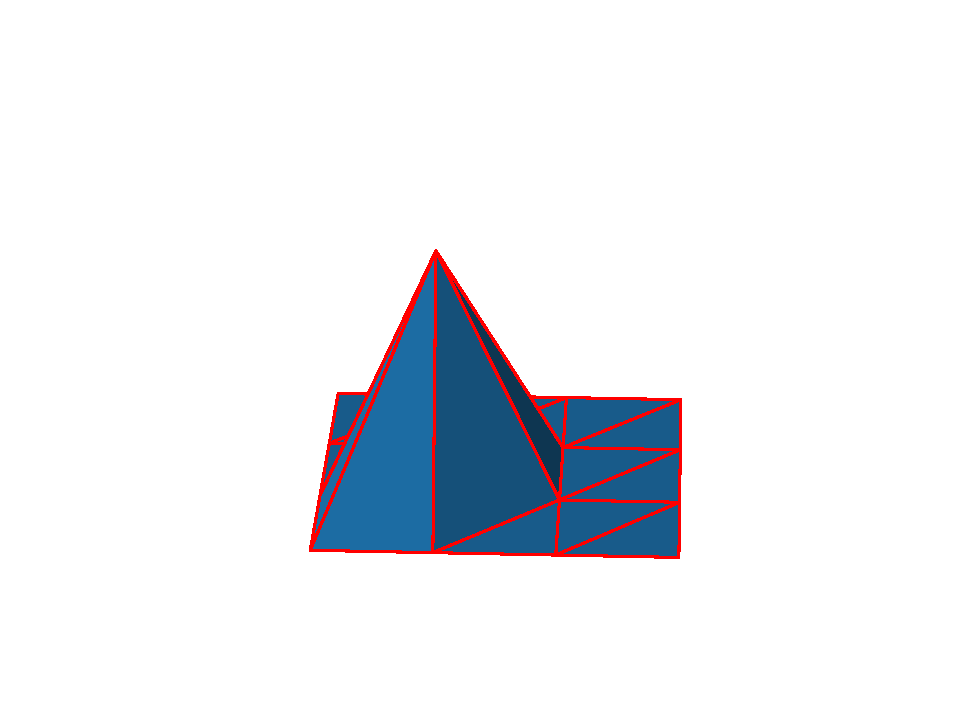
\includegraphics[width=0.8\textwidth]{hat_function_python_plot_2.pdf}
		\caption{A hat function .}
		\label{fig:hat1}
	\end{figure}
	Now, we demonstrate how the method works in practice. We seek a solution $u_h \in V_h$. Write this in terms of the basis functions: $u_h = \sum_{i=1}^n \hat{u}_i \phi_i$. Now, \eqref{eq:galerkin} can be written as an equation with a solution vector with real coefficients: Find $\hat{\bm{u}}_h$ in $\mathbb{R}^n$ such that
	\begin{equation}\label{eq:fem system}
		\begin{gathered}
			\sum_{i=1}^n \hat{u}_i  a(\phi_i,\phi_j) = b(\phi_j).
		\end{gathered}
	\end{equation}
	So we get a system of linear equations $\bm{A}\hat{\bm{u}}_h = \bm{b}$, where we have one equation for each interior node. If we solve \eqref{eq:variational poisson}, our variational problem, and also matrix, will be symmetric. The matrix is then often called a \emph{stiffness matrix}. These names originated from mechanics and structural analysis, where the solution represents displacement and the force function represents load. The stiffness matrix is also sparse, which is a very important property when designing algorithms to solve it.\par
	With the setup described in this subsection, the degrees of freedom are the same as the dimension of $V_h$. If we in definition \ref{def:linear ansatz} instead had chosen a space of quadratic polynomials on each element, we hade gained three degrees of freedom on each element. In this thesis we focus on linear finite elements because we do not gain anything from increasing regularity, as the solutions are not expected to be very regular. 
	\subsection{Implementation}
	\addcontentsline{toc}{subsection}{Implementation}
	In this subsection we explain the most important parts of the algorithm for discretizing elliptic PDE's with linear triangular elements. We consider the homogenous elliptic model problem \eqref{eq:variational poisson} in two dimensions with $\bm{K} = \bm{I}$. The procedure goes as follows:
	\begin{enumerate}
		\item Make a triangulation of the domain. This can be done in a number of different ways, see chapter 4 of Knabner \cite{Knabner}. If we have $N$ nodes, our triangulation would be stored as a $N \times 2$ array of floats, being the coordinates of the nodes. And a $E\times 3$ array of ints being the elements, where each entry is the index of a coordinate in the coordinate matrix, E is the number of elements.
		\item Allocate space for the $N \times N$ stiffness matrix $\bm{A}$ and the $N \times 1$ source vector $\bm{b}$.
		\item Define the basis functions on a reference element, this is also called the shape functions, see figure \ref{fig:reference element} and \eqref{eq:shape functions}. Also compute the gradients of the shape functions. 
		\begin{equation}
			\begin{gathered}\label{eq:shape functions}
				N_1(x,y) = 1-x-y\\
				N_2(x,y) = x\\
				N_3(x,y) = y
			\end{gathered}
		\end{equation}
		\begin{figure}[H]
			\centering
			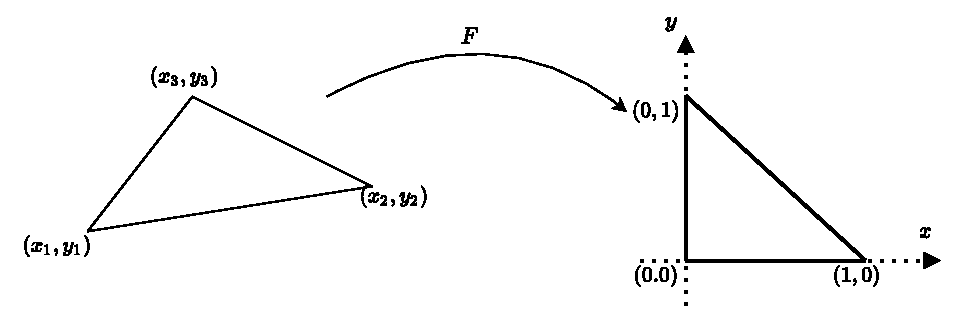
\includegraphics[width=0.85\textwidth]{reference element.pdf}
			\caption{The map $F$ from element $K$ to the reference element $\hat{K}$.}
			\label{fig:reference element}
		\end{figure}
		\item Loop through the elements. For each element $K$ compute the affine linear map that maps it to the reference element. That means we want to find $B\in \mathbb{R}^{2\times 2}$ and $d\in \mathbb{R}^2$ such that 
		\begin{equation}
			\begin{aligned}
				F: K &\rightarrow \hat{K}\\
				x &\mapsto B x + d
			\end{aligned}
		\end{equation}
		To achieve this we set up a system of equations inspired by figure \ref{fig:reference element}
		\begin{gather}\label{eq:find_Bd}
			\begin{pmatrix}
				x_1 & y_1 & 1\\ 
				x_2 & y_2 & 1\\ 
				x_3 & y_3 & 1
			\end{pmatrix}\begin{pmatrix}
				b_{1,1} & b_{2,1}\\ 
				b_{1,2} & b_{2,2}\\ 
				d_1 & d_2
			\end{pmatrix}=
			\begin{pmatrix}
				0 &0 \\ 
				1& 0\\ 
				0 &1 
			\end{pmatrix}
		\end{gather}
		So for each element we solve \eqref{eq:find_Bd} for $B$ and $d$, that means computing an inverse of a three by three matrix and a matrix product. Note that this only needs to be done once and could be done in a preprocessing step. \par
		Now that we have $T$, we do the following on the element:
		\begin{enumerate}
					\item Use the map and the shape functions to evaluate $a(\phi_i,\phi_j)|_K$  for $1\leq i,j \leq 3$. Note that for $u: K \rightarrow \mathbb{R}$ we get by the chain rule:
			\begin{equation}
				\nabla^T_{\hat{x}} u(F^{-1}(\hat{x})) = \nabla^T_{x}u(F^{-1}(\hat{x}))\nabla^T_{\hat{x}} F^{-1}(\hat{x}) =\nabla^T_{x}u(F^{-1}(\hat{x})) B^{-1}.
			\end{equation}
			This gives an expression for the derivative on an element expressed as a derivative in the reference element coordinate system:
			\begin{equation}
				\nabla_{x}u(F^{-1}(\hat{x})) = B^T \nabla_{\hat{x}} u(F^{-1}(\hat{x})).
			\end{equation}
			Now we can compute the product of the gradients of the basis functions on an element:
			\begin{equation}\label{eq:elementgradient}
				\begin{aligned}
					a(\phi_i,\phi_j)|_K &= \int_K (\nabla \phi_i)^T \nabla \phi_j dx\\
					&= \int_{\hat{K}} (\nabla_x \phi_i(F^{-1}(\hat{x})))^T\nabla_x \phi_j(F^{-1}(\hat{x})) |\text{Det}(J(F^{-1}))|d\hat{x}\\
					&=\int_{\hat{K}}(B^T \nabla_{\hat{x}}\phi_i (F^{-1}(\hat{x})))^TB^T B \nabla_{\hat{x}}\phi_j (F^{-1}(\hat{x})) |\text{Det}(B^{-1})|d\hat{x}\\
					&=\int_{\hat{K}} (\nabla_{\hat{x}}N_i(\hat{x}))^TB^TB\nabla_{\hat{x}} N_j(\hat{x}) |\text{Det}(B^{-1})|d\hat{x}\\
					&= \frac{1}{2} (\nabla_{\hat{x}}N_i(\hat{x}))^TB^TB\nabla_{\hat{x}} N_j(\hat{x}) \frac{1}{|\text{Det}(B)|}
				\end{aligned}
			\end{equation}
			So for each element we evaluate the last line of \eqref{eq:elementgradient} for all(9) combinations of $i$ and $j$ on the element 
			and add this to $\bm{A}_{i,j}$. This approach is called \emph{element-based assembling}, and $\bm{A}_{i,j} = \sum_{K\in \mathcal{N}(i)} a(\phi_i,\phi_j)|_K$, where $\mathcal{N}(i)$ is the set of all elements that contain node $i$.
			\item In almost the same way we compute $b(\phi_i)|_K$ and add this to $\bm{b}_i$. As in \eqref{eq:elementgradient} we compute the integral on the reference element:
			\begin{equation}
				\begin{aligned}
					b(\phi_i)|_K &= \int_{\hat{K}} f(F^{-1}(\hat{x})) \phi_i(F^{-1}(\hat{x})) \frac{1}{\text{Det}(B)}d\hat{x}\\
					&= \int_{\hat{K}}\hat{f}(\hat{x}) N_i(F^{-1}(\hat{x}))\frac{1}{\text{Det}(B)}d\hat{x}\\
					&\approx \frac{1}{\text{Det}(B)} \sum_k \omega_k \hat{f}(\hat{p}_k) N_i(\hat{p}_k)
				\end{aligned}
			\end{equation}
			Where $\hat{f}:= f(F^{-1}(\hat{x}))$ and $\left \{ (\omega_k,\hat{p}_k) \right \}_k$ defines a \emph{quadrature rule}. We will see later that this quadrature rule can be chosen in different ways, for higher order finite elements this may even affect the convergence behaviour. 
		\end{enumerate}

		\item Loop through the nodes $x_j$ at the boundary and set $\bm{A}_{j,i}=\delta_{ij}$, $b_j = 0$

	\end{enumerate}
	\begin{remark}
		If we have inhomogeneous Dirichlet boundary conditions this is in practice done the same way as in the homogenous case, eliminating the degrees of freedom on the boundary. For Neumann conditions one has to evaluate integrals along the boundary as in \eqref{eq:inhomogenous poisson weak}, using one-dimensional elements.
	\end{remark}
	\subsection{Convergence}\label{sec:convergence}
	\addcontentsline{toc}{subsection}{Convergence}
	
	In this subsection, we review the most important concepts in studying the convergence fo FEM, for a detailed discussion see \cite{Knabner}.
	The starting point of convergence estimates for the finite element method already described are \textbf{Cèa's lemma}:
	\begin{theorem}[Cèa's lemma]
		Let $u$ solve the variational problem \eqref{eq:variational problem} and $u_h$ solve the corresponding Galerkin approximation \eqref{eq:galerkin}, where the bi linear form $a$ is bounded and coercive. Then we have:
		\begin{equation}
			\left \| u-u_h \right \|_V \leq \frac{C_b}{C_c}\text{min} \left \{ \left \| u-v_h \right \|: \ v_h \in V_h \right \}.
		\end{equation}
		
	\end{theorem}
	\begin{proof}
		By the coercivity and linearity of $a(\cdot,\cdot)$ we have:
		\begin{equation*}
			C_c \left \| u-u_h \right \|^2_V \leq a(u-u_h,u-u_h) = a(u-u_h,u-v_h) + a(u-u_h, v_h - u_h).
		\end{equation*}
		The last term equals zero, since both $u$ and $u_h$ solves the variational problem in $V_h$: $v_h-u_h = v \in V_h$ and $a(u-u_h,v) = a(u,v)-a(u_h,v) = b(v)-b(v) = 0$, this is called \emph{Galerkin orthogality}. Hence we only need to use the boundedness of $a(\cdot,\cdot)$:
		\begin{equation*}
			C_c \left \| u-u_h \right \|^2_V \leq a(u-u_h,u-u_h) \leq C_b \left \| u-u_h \right \|_V \left \| u-v_h \right \|_V.
		\end{equation*}
		We divide by $C_c$ and $\left \| u-u_h \right \|_V$ and take the infimum over $v_h \in V_h$:
		\begin{equation*}
			\left \| u-u_h \right \|_V \leq \frac{C_b}{C_c} \text{inf} \left \{ \left \| u-v_h \right \|_V: v_h \in V_h \right \}.
		\end{equation*}
		By (Cheney \cite{Cheney}, page 64, theorem 2), as $V_h$ is closed and convex subspace of a Hilbert space, there exist an unique element of $V_h$ closest to $u$ and minimum is attained.  
	\end{proof}
	Hence the solution to Galerkin problem is the best in the subspace $V_h$ up to a constant. We can therefore study convergence rate estimates for a suitable comparison element in $V_h$. In one dimension it is easy to picture what this comparison element might be, see figure \ref{fig:1dinterpolation}. A direct proof with techniques from calculus is possible in this case.\\
	\begin{figure}[H]
		\centering
		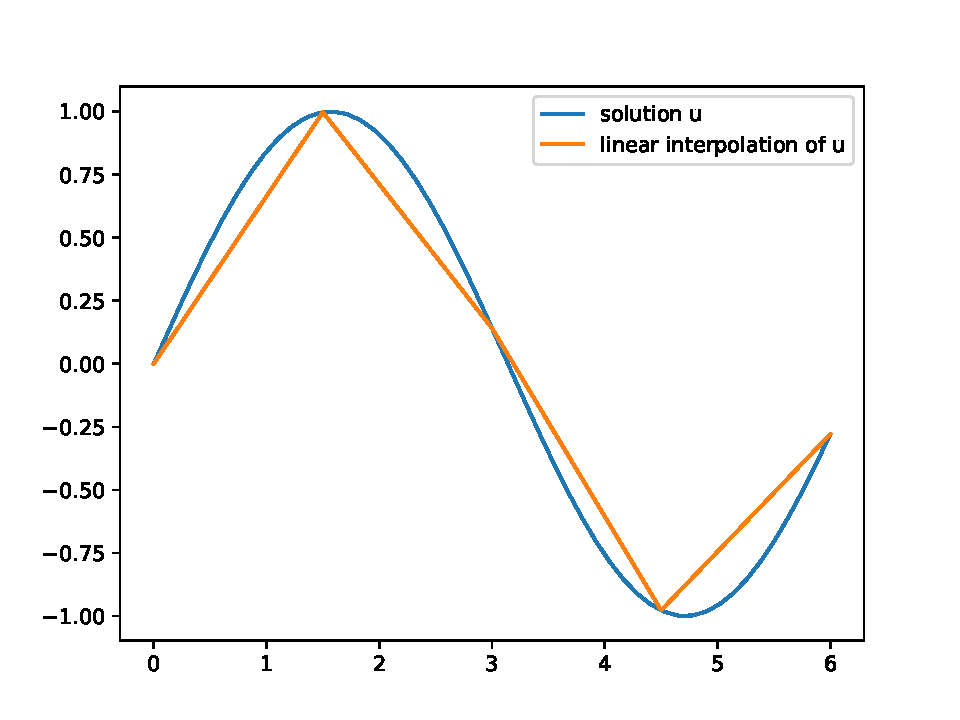
\includegraphics[width=0.7\textwidth]{interpolation.pdf}
		\caption{The unique linear interpolation of a function in one dimension.}
		\label{fig:1dinterpolation}
	\end{figure}
	The idea for more dimensions are the same, to be precise we define the interolation operator.
	\begin{definition}[Global interpolation operator]		\label{def:global_interpolator}
		\begin{gather*}
			I_h:C(\overline{\Omega}) \rightarrow V_h \\
			v \mapsto \sum_{i}v(n_i) \phi_i
		\end{gather*} 
	Where $\left\{ n_i\right \}_i$ are the nodes and $\left\{ \phi_i\right \}_i$ the corresponding basis functions.

	\end{definition}
	\begin{remark}
		The global interpolator operator \ref{def:global_interpolator} maps from continuous functions, so we need to make sure our solution is continuous. By the Sobolev embedding theorem, (Evans \cite{evans10},page 286) we are okay if our space dimension is below three and $u \in H^k(\Omega)$ for $k\geq 2$.
	\end{remark}
	Hence, in the setting of the model problem \eqref{eq:variational poisson}, we hope to reach an estimate on the form
	\begin{equation}\label{eq:energy norm estimate}
		\left \| u-u_h \right \|_{1} \leq C \left \| u-I_h(u) \right \|_{1}\leq C^* h^{k}|u|_{k+1}
	\end{equation}
	Where $h$ is the maximum diameter of the elements in the triangulation, and $k$ is the polynomial degree on the ansatz space.
	This bound is indeed attainable if we make sure the triangles in our triangulation have maximum angle less than $\pi$.
	In chapter 3.4 of Knabner \cite{Knabner}, there is a detailed proof of \eqref{eq:energy norm estimate}.\\
	Note that this means that our linear finite element method has a linear convergence in the $\left \| \cdot \right \|_1$ norm, if our variational problem admits a solution with sufficient regularity. We tie these observations together in a theorem:
	\begin{theorem}[energy norm estimate]\label{th:energy error estimate}
		Consider a finite element discretization as described by \eqref{eq:fem system} in $\mathbb{R}^d$ for $d\leq 3$ on a family of triangulations with an uniform upper bound on the maximal angle. Suppose we have a linear ansatz space as in \ref{def:linear ansatz}, then
		\begin{equation}
			\left \| u-u_h \right \|_{1}\leq C h|u|_{2}.
		\end{equation}
	\end{theorem}
	Often we are happy with a convergence rate estimate in the $\left \| \cdot \right \|_0$ norm, which do not measure an error in the approximation of the derivative. We then expect a better convergence rate, as can be shown by the \emph{duality trick}. We consider the dual problem of our variational problem \eqref{eq:variational poisson}: $a(v,u_f) = \left \langle f,v\right \rangle_0$, and assume some uniqueness and stability of the solution $u_f$ of this. 
	\begin{theorem}[$L^2$ estimate]
		Suppose the situation of theorem \ref{th:energy error estimate} and assume there exist an unique solution to the adjoint problem with $| u_f| \leq C \left \|f \right \|_0$, then there exist a constant $C^*$ such that:
		\begin{equation}
			\left \| u - u_h \right \|_0 \leq C^* h \left \| u- u_h \right \|_1.
		\end{equation}
	\end{theorem}
	See \cite{Knabner} for a proof. When it comes to the assumption on the dual problem, this is satisfied for our elliptic model problem \ref{eq:poisson}. If we put the last two theorems together we obtain quadratic convergence in the $L^2$ norm
	\begin{remark}
		In this chapter we have only discussed the convergence behaviour of the solution to the Galerkin problem \eqref{eq:galerkin}. In practice, one often only solves this approximately. For example the term  $b(v_h)=\int_{\Omega}fv_h \ dx$ is impossible to evaluate exactly for most source terms $f$. We will later see error estimates with this taken into account.
	\end{remark}
	\section*{Finite Volume Method}
	\addcontentsline{toc}{section}{Finite Volume Method}

		Finite volume methods are designed such that the conservation law we solve hold everywhere in the domain. Consider our elliptic model problem \eqref{eq:poisson}:
		Find $u$ such that:
		\begin{equation} 
			\begin{split}
				-\nabla \cdot \bm{K} \nabla u(x) &= f(x) \ \  x\in \Omega \\ 
				u(x) &= 0 \ \ x\in \partial \Omega.
			\end{split}
		\end{equation}
		
		 First we divide our domain $\Omega$ into convex quadrilaterals (control volumes, cells), $\left \{ \Omega_i \right \}_i$. Then we integrate our equation over $\Omega_i$ and use the divergence theorem:
	\begin{equation}\label{eq:fvm1}
		\int_{\Omega_i} -\nabla \cdot \bm{K} \nabla u dx = -\int_{\partial \Omega_i} \bm{K}\nabla u \cdot \bm{\hat{n}} ds = \int_{\Omega_i}fdx
	\end{equation}
	The above equation equates the fluxes through the boundary of a control volume, with the source or sinks inside the control volume. The finite volume methods are discrete versions of this. Let $E_{i,j}$ be the the edge between cells $i$ and $j$. Then the main idea is to approximate the flux through $E_{i,j}$, from cell $i$ to cell $j$,
	\begin{equation}
		q_{E_{i,j}} =-\int_{E_{i,j}} \bm{K}\nabla u \cdot \bm{\hat{n}} ds
	\end{equation}
	
	by a linear combination of $u_i$ at neighbouring cell centers
	\begin{equation}
		q_{E_{i,j}}\approx \tilde{q}_{E_{i,j}} = \sum_{k}t_{i,j}^k u^k.
	\end{equation}
	Where the \emph{transmissibility } $t_{i,j}^k$ has the property $\sum_k t_{i,j}^k = 0$. Note that with this notation, we have $q_{E_{i,j}} = - q_{E_{j,i}}$.\par
	We also approximate the integral on the right side, $\int_{\Omega_i}fdx$, with some quadrature rule. In porous media flow, the space discretization used, usually have a truncation error of at most second order. This has to do with the regularity of the solution due to heterogeneous permeability. The upshot is that we use the midpoint rule for evaluating the right hand side, as this also has a second order truncation error. Hence we evaluate $f$ at the cell center and multiply by the area of $\Omega_i$. We then end up with a system of equations
	\begin{equation}\label{eq:fvm system}
		\sum_{j\in \mathcal{S}_i} \tilde{q}_{E_{i,j}} = |\Omega_i|f(x_i),
	\end{equation}
	where $\mathcal{S}_i$ is the set of indexes of neighbouring cells.
	The system of equations \eqref{eq:fvm system} ensures local mass conservation. It can also be written in matrix form as:
	\begin{equation}
		\bm{A}^V\tilde{\bm{u}}_h = \bm{f}.
	\end{equation}
	 We will discuss different ways of constructing the transmissibility coefficients, as they result in very different discretizations.
	\par
	The motivation for using finite volume methods for problems in porous media, for example Richards' equation, is that the flux appears explicitly in our discretization. If one, for example, wants to simulate the spread of some contaminant by groundwater flow, one can easily obtain a local mass conservative flux field using the finite volume method. This flux field can then be coupled with the desired transport equation.
	\par 
	When it comes to boundary conditions, this is usually straightforward for Neumann boundaries. Especially no-flow boundary conditions, where one makes creates a strip of cells outside the boundary with zero permeability. The same discretization algorithm can the be applied everywhere in the domain. Dirichlet boundary conditions often require more special care. If one, however, knows the solution somewhere outside the domain, one could make a strip of cells outside the boundary where the potential values are known, this is known as ghost Dirichlet boundary conditions. We will focus on discretizing the interior of the domain in the following sections.
	\subsection*{Two point flux approximation}
	\addcontentsline{toc}{subsection}{Two point flux approximation}The simplest way of constructing $t_{i,j}^k$ is also the most popular in the industry. As the name suggests, we only use the function value at two points, $x_{0}$ and $x_{1}$, to compute the numerical flux $\tilde{q}_{E_{0,1}}$.
	\begin{figure}[H]
		\centering
		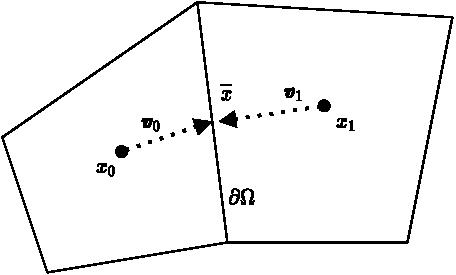
\includegraphics[width=0.5\textwidth]{two point.pdf}
		\caption{The two point flux approximation (TPFA) setup.}
		\label{fig:tpfa control volume}
	\end{figure}
	Let $\bm{v}_1$ be the vector from cell center $x_0$ to the midpoint of the edge between the cells, $\overline{x}$. Then we approximate the flux out of cell $x_0$ into cell $x_1$ by:
	
	\begin{equation}\label{eq:f_0}
		\tilde{q}_{E_{0,1},0}=-\bm{n}_0^T \bm{K}_0  \frac{\bm{v}_0}{\left \| \bm{v}_0 \right \|} (u(\overline{x})-u(x_0))ds
	\end{equation}
	
	or as
	
	\begin{equation}\label{eq:f_1}
		\tilde{q}_{E_{0,1},1} = -\bm{n_1}^T \bm{K}_1  \frac{\bm{v}_1}{\left \| \bm{v}_1 \right \|} (u(x_1)-u(\overline{x}))ds
	\end{equation}	
	
	where $\hat{\bm{n}_i}$ is the normal vector pointing out of cell $i$ with length equal to $\partial \Omega$.
	Because we require flux continuity we have that 
	\begin{equation}
		\tilde{q}_{E_{0,1},0} = \tilde{q}_{E_{0,1},1} = t^0 u(x_0) + t^1 u(x_1)
	\end{equation}
	where, as before, $t^0 + t^1 = 0 \Rightarrow t^0 = -t^1$, and the subscript on $t$ is dropped for readability. We now have three equations and three unknowns, $u(\overline{x})$, $t^0$ and $t^1$. To simplify, we introduce the quantity $T_i := \bm{n}_i^T \bm{K}_i  \frac{\bm{v}_i}{\left \| \bm{v}_i \right \|} $ to represent the cell transmissivity. So first we solve for $u(\overline{x})$:
	\begin{equation}
		T_0(u(\overline{x})-u(x_0)) = T_1(u(x_1)-u(\overline{x})) \Rightarrow u(\overline{x}) = \frac{T_0 u(x_0) + T_1 u(x_1)}{T_0 + T_1}.
	\end{equation}
	Next we insert this into the expression for $\tilde{q}_0$:
	\begin{equation}
		\begin{aligned}
			\tilde{q}_{E_{0,1},0} =& -T_0(u(\overline{x})-u(x_0)) \\
			=& -T_0\left (\frac{T_0 u(x_0) + T_1 u(x_1)}{T_0 + T_1} - u(x_0)\right )\\
			=& -T_0\left (\frac{T_0 u(x_0) + T_1 u(x_1) - u(x_0)T_0 - u(x_0)T_1}{T_0 + T_1}\right ) \\
			=& -T_0\left (\frac{ T_1 u(x_1)  - u(x_0)T_1}{T_0 + T_1}\right)\\
			=& \frac{u(x_0)-u(x_1)}{\frac{1}{T_1} + \frac{1}{T_0}}.
		\end{aligned}
	\end{equation}
	Now, we have solved the equations for the transmissivity coefficients:
	\begin{equation}\label{eq:harmonic mean}
		\begin{aligned}
			\tilde{q}_{E_{0,1},0} &= t^0 u(x_0) + t^1 u(x_1) \\
			\frac{u(x_0)-u(x_1)}{\frac{1}{T_1} + \frac{1}{T_0}} &= t^0 u(x_0) + t^1 u(x_1) \\
			\Rightarrow t^0 &= \frac{1}{\frac{1}{T_1} + \frac{1}{T_0}}.
		\end{aligned}
	\end{equation} 
	Hence, the transmissibility is the \emph{harmonic mean} of the local transmissivities. One way of looking at this discretization, is that we assume the potential to be a linear function of one variable in the $v_i$ direction between the cell center and the edge in figure \ref{fig:tpfa control volume}. So for each edge, we have two linear functions on each side, which gives us four degrees of freedom. Two of them are used to respect the cell center potential values, the other two are used on pressure and flux continuity across the edge. With these assumptions, expressions \eqref{eq:f_0} and \eqref{eq:f_1} are exact. And we only have to solve for the transmissibility coefficients.\par
	 Two point flux approximation has the advantage of being fast to assemble and simple to code. It yields a pleasant five point stencil for two dimensional problems. However, there is one big disadvantage with two point flux approximation: Computing the flux with only two points is not consistent when the grid is not aligned with the principal directions of $\bm{K}$. If our grid is aligned with $\bm{K}$, we have that 
	\begin{equation}
		\bm{n}_2 \cdot \bm{K}\bm{n}_1 = 0
	\end{equation}
	for a uniform parallelogram mesh with the normal vectors $\bm{n}_1$ and $\bm{n}_2$. We then call the grid \textbf{K-orthogonal}. 
	 In the setting of figure \ref{fig:tpfa control volume}, our grid would not be K-orthogonal as the control volumes are not a parallelograms. All meshes with orthogonal control volumes are K-orthogonal if the permeability is isotropic.
	 \todo[inline]{reference a figure showing the failed convergence of TPFA}
	\subsection*{O-method}
	\addcontentsline{toc}{subsection}{O-method}
	The O-method is a multi-point flux approximation method, these types of methods were developed to make control volume methods converge for grids that are not K-orthogonal. It is described in detail in  \cite{Aavatsmark2002}, we only give a brief introduction.
	\\
	Consider the control volumes in \ref{fig:dualmesh}.
	\begin{figure}[H]
		\centering
		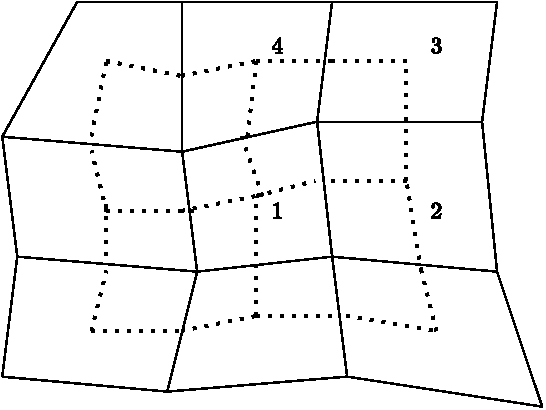
\includegraphics{dualmesh.pdf}
		
		\caption{The solid lines are the control volumes, the dashed lines are the dual mesh connecting the cell centers, going through the midpoints of each edge. The solid circles are cell centers, the white circles are grid points .}
		\label{fig:dualmesh}
	\end{figure}
	For each grid point, that means where four control volumes intersect, we consider an interaction region. This is the polygon drawn by the dual mesh around the grid point.
	\begin{figure}[H]
		\centering
		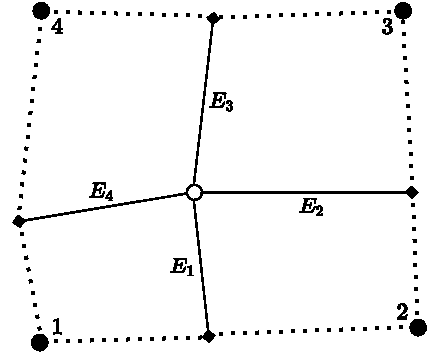
\includegraphics[width=0.6\textwidth]{Interaction region.pdf}
		\caption{The four subcells in the interaction region corresponding to cells $1,2,3,4$ and grid point $5$. Here, $\mathcal{R}_5 = \left \{1,2,3,4 \right\}$.}
		\label{fig:interactionregion}
	\end{figure}
	In each interaction region there are four half edges. Our goal is to obtain an expression 
	\begin{equation}\label{eq:O trans}
		\tilde{q}_{E_{i,j}}^n  = \sum_{k\in \mathcal{R}_n} t^{k,n}_{i,j} u^k  \approx \int_{E_{i,j}}\hat{\bm{n}}_j^T \bm{K} \nabla u \  ds \ \ i,j \in \mathcal{R}_n
	\end{equation}
	for the flux through each half edge $E_{i,j}^n$ in the interaction region corresponding to grid point $n$ (figure \ref{fig:interactionregion}). Where $\mathcal{R}_n$ is the index set of the four cells neighbouring grid point $n$.
	\par
	We assume for now that the potential is linear in each of the four sub cells in the interaction region, figure  \ref{fig:interactionregion}. This gives $4\cdot 3 = 12$ degrees of freedom. The linear potential must of course equal the cell center values of the potential in the cell centres, this removes four degrees of freedom. We also require flux continuity on the four half edges in the interaction region, this removes an additional four degrees of freedom. The last four degrees of freedom are spent on potential continuity of the midpoints of the edges. 
	\par
	By these assumptions on flux and potential continuity, the linear potential in each sub cell is well defined given values at the cell center. We can now use this to compute the four by four matrix of transmissibility coefficients for each of the four half edges. In the situation of figure \ref{fig:interactionregion} and equation \eqref{eq:O trans} it would look like
	\begin{equation}\label{eq:O trans matrix}
		\bm{T}^5 = \begin{bmatrix}
			t^{1,5}_{1,2} &t^{2,5}_{1,2} &t^{3,5}_{1,2}  &t^{4,5}_{1,2} \\ 
			t^{1,5}_{2,3} &t^{2,5}_{2,3}  &t^{3,5}_{2,3}  &t^{4,5}_{2,3} \\ 
			t^{1,5}_{4,3} & t^{2,5}_{4,3} & t^{3,5}_{4,3} & t^{4,5}_{4,3}\\ 
			t^{1,5}_{1,4} & t^{2,5}_{1,4} & t^{3,5}_{1,4} & t^{4,5}_{1,4}
		\end{bmatrix}.
	\end{equation}
Computing \eqref{eq:O trans matrix} involves inverting a four by four matrix with coefficients depending on the mesh and permeability, see \cite{Aavatsmark2002} for details. Finally, we assemble the system of equations \eqref{eq:fvm system} with the transmissibility coefficients. Note that we write the flux over the $j$th edge of cell $i$, $\tilde{q}_{i,j}$ as the flux over the two half edges:
	\begin{equation*}
		\begin{aligned}
			\sum_{j\in \mathcal{S}_i} (\tilde{q}_{E_{i,j}}^1 + \tilde{q}_{E_{i,j}}^2) &= |\Omega_i|f(x_i) \\
			\sum_{j=1}^4 (\sum_{k=1}^4 t^{k,1}_{i,j}u^k + \sum_{k=1}^4 t^{k,2}_{i,j}u^k)&= |\Omega_i|f(x_i).\\
		\end{aligned}
	\end{equation*}
	Next, we see that the interaction regions of the two half edges sharing same edge overlaps, so we get a six point flux stencil:
	\begin{equation*}
		\sum_{j=1}^4 \sum_{k=1}^6 \overline{t}^{k}_{i,j}u^k = |\Omega_i|f(x_i).
	\end{equation*}
	We can simplify this further and see that we get a nine point stencil:
	\begin{equation*}
		\sum_{k=1}^9 \hat{t}^{k}_{i,j}u^k = |\Omega_i|f(x_i).
	\end{equation*}
	The O-method is consistent for non K-orthogonal grids, and reduces to two point flux approximation when the grid is K-orthogonal. This happens because the systems of equations to be solved for the transmissibility coefficients in each interaction region, becomes diagonal. This is because $\bm{n}^T \bm{K} \nabla u$ can be expressed as two points when $u$ is given by three points which are K-orthogonal.
	\par
	In \cite{nordbotten2020introduction}, Nordbotten and Keilegavlen describes a framework of MPFA methods where the O-method is a special case. They consider the problem of finding the four linear potential functions in each interaction region that minimizes the discontinuity across the edges. The discontinuity should be minimized given that the functions respect cell center potential values, that the flux models the constitute law and flux continuity. The O-method is then defined for some special cost function measuring the discontinuity. Other methods, with the potential continuity at other places than the edge midpoint, are also common.
	\par 
	With my implementation of MPFA-O method, one needs for each interaction region to assemble four, four by four, matrices. Compute the inverse of one of them, and do two matrix multiplications and one subtraction. All of this could be done in parallel. However, for my implementation, it slows matrix assembly down a lot compared to two point flux approximation. Another drawback of the O-method is the \emph{monotonicity} properties: One can risk having positive entries off the main diagonal of the discretization matrix for difficult meshes. This may lead to oscillations in the solution and violation of the minimum principle. For two point flux approximation we avoid this issue altogether, as the signs of the five point stencil always are one plus and four negatives. Even for the linear finite element method, this issue is avoided if one imposes some maximum angle condition, see [Knabner,\cite{Knabner}] page 175. When solving for example the Richards' equation, violating the minimum principle can lead to air bubbles being formed spontaneously in the saturated region. For a discussion on monotonicity see \cite{10.1007/s00211-006-0060-z}.
	\subsection*{L-method}
	\addcontentsline{toc}{subsection}{L-method}
	\epigraph{The L-method is the Ferrari of discretization techniques for porous media flow problems, while conformal finite elements is the Volvo.}{\textit{Professor Jan Martin Nordbotten}}
	As the O-method, the L-method is also a multipoint flux approximation method. It was introduced in \cite{https://doi.org/10.1002/num.20320}, where the authors demonstrate improved monotonicity properties with numerical experiments. This method is similar to the O-method, in that it goes through the half edges and uses information from the same interaction regions. But instead of using four points for the flux across each half edge, we use three, with two half edges between them. \par
	As in the O-method, we assume linear potential in each cell, this gives us $3\cdot 3 = 9$ degrees of freedom. Three are eliminated because we respect the cell center value of the potential, this leaves six degrees of freedom. We use two, one at each edge, for flux continuity. The last four are used for potential continuity at the two edges. 
	\par
	We have two choices of flux stencil for each half edge, see figure \ref{fig:two choices}. We compute the transmissibility coefficients for both, then we choose the one "best" aligned with the flow: Let $t_1^i$ be the $i$th transmissibility coefficient of $T_1$, then
	\begin{equation}\label{eq:L-criterion}
		\begin{aligned}
			&\text{if} \ |t^1_1| < |t^2_2| \\
			&\text{choose} \ T_1 \ \text{else} \\
			&\text{choose} \ T_2.
		\end{aligned}
	\end{equation}
	\begin{figure}[H]
		\centering
		\begin{subfigure}[b]{0.4\textwidth}
			\centering
			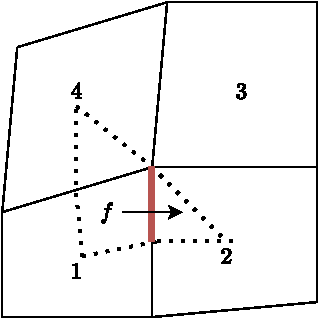
\includegraphics[width=\textwidth]{left choice.pdf}
			\caption{$T_1$}
		\end{subfigure}
		\hfill
		\begin{subfigure}[b]{0.4\textwidth}
			\centering
			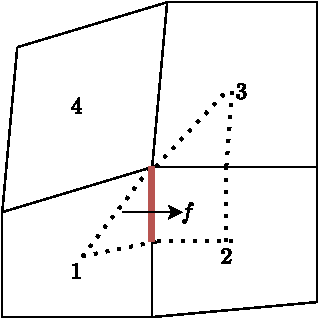
\includegraphics[width=\textwidth]{right choice.pdf}
			\caption{$T_2$}
			\label{fig:three sin x}
		\end{subfigure}
		\caption{The two choices of which cell centers to use for computing the flux over the half edge in red. We call the triangles spanned $T_1$ and $T_2$ for L-triangles.}
		\label{fig:two choices}
	\end{figure}
	A cheap intuition behind \eqref{eq:L-criterion} is that if $|t_1^1|<|t_2^2|$, it is more likely that $sgn(t_1^1) = sgn(t_1^4)$ and if not, $sgn(t_2^2) = sgn(t_2^3)$ is more likely. This is due to the fact that $\sum t^i = 0$. Choosing L-triangle as in \eqref{eq:L-criterion} increases the chances that we get the same sign of $t^i$ on the same side of the half edge, thus increasing the chance that we get a monotone discretization.  See \cite{https://doi.org/10.1002/fld.1926} for a more detailed geometric intuition of choosing L-triangle in the case of homogenous permeability. 
	\par 
	To compute transmissibility coefficients in a given L-triangle, we use the assumptions on flux and potential continuity, to construct a linear system. The coefficients depends on mesh and permeability in the three cells. In general, we need to solve two linear systems for each half edge, as there are always two choices. In the O-method it is enough to solve a linear system per four half edges.
	
	\par
		As with the O-method, we end up with a system assembled from the fluxes over the half edges:
	\begin{equation}
		\begin{aligned}
			\sum_{j=1}^4 (\tilde{q}_{i,j}^1 + \tilde{q}_{i,j}^2) &= |\Omega_i|f(x_i) \\
			\sum_{j=1}^4 (\sum_{k=1}^3 t^{k,1}_{i,j}u^k + \sum_{k=1}^3 t^{k,2}_{i,j}u^k)&= |\Omega_i|f(x_i).\\
		\end{aligned}
	\end{equation}
	But the flux stencil across each edge is possibly smaller, often just four points.
	\par
	In figure \ref{fig:L-triangles} we see the criterion in practice for a homogenous medium: In figure \ref{fig:paralellogram-L} all L-triangles are used by two half-edges, and they are chosen in the same way throughout the domain. In figure \ref{fig:complicated-L} there are some triangles that overlap, this is due to the fact that some L-triangles are used by only one half edge.
	\begin{figure}[H]
		\centering
		\begin{subfigure}[b]{0.8\textwidth}
			\centering
			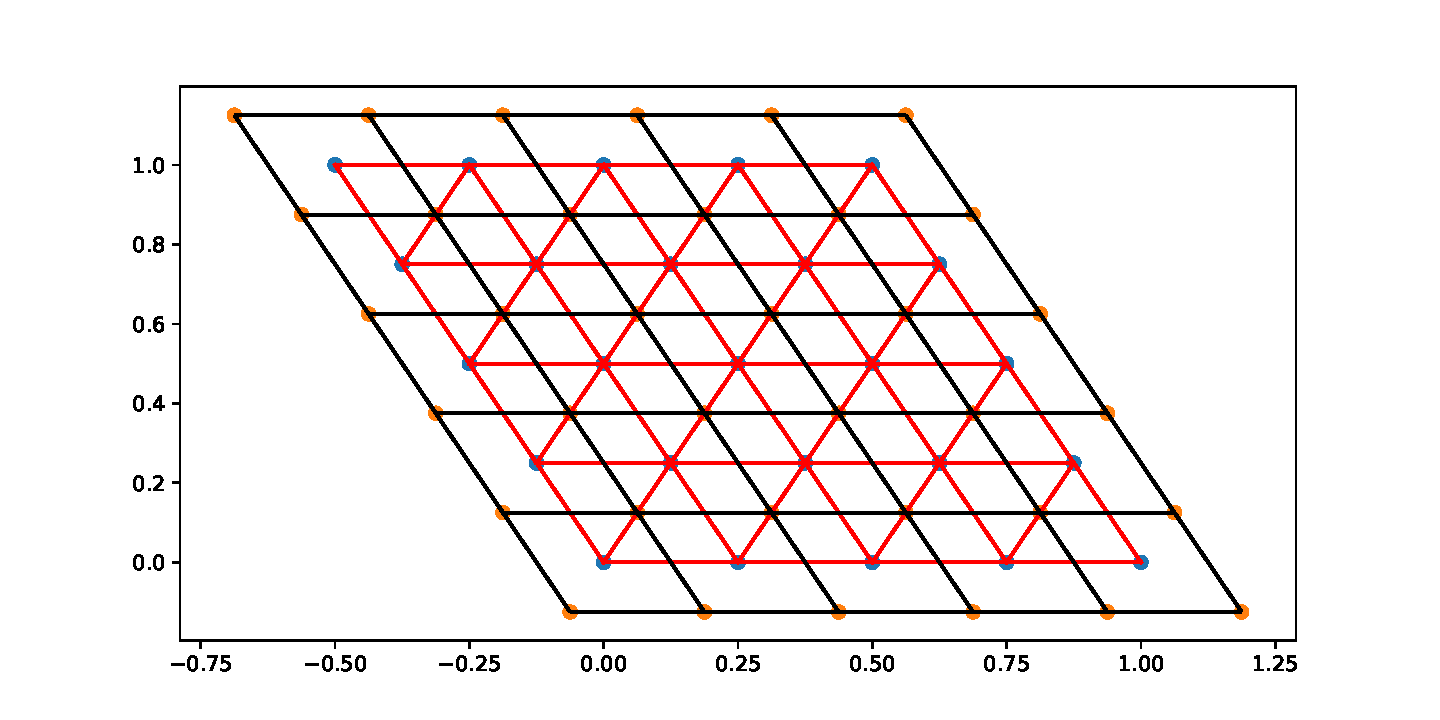
\includegraphics[width=\textwidth]{L-triangles_paralellogram.pdf}
			\caption{Parallelogram grid, all triangles are chose similarly.}
			\label{fig:paralellogram-L}
		\end{subfigure}
		\hfill
		\begin{subfigure}[b]{0.8\textwidth}
			\centering
			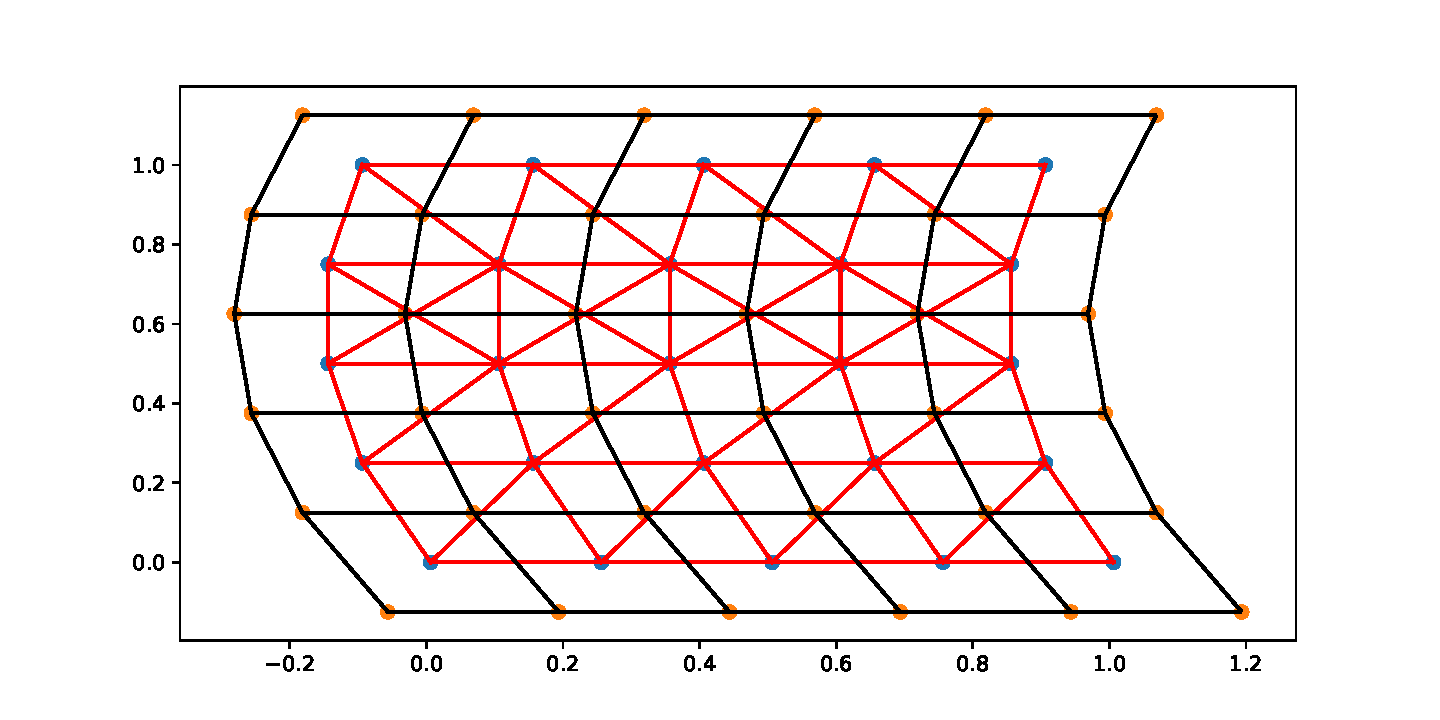
\includegraphics[width=\textwidth]{L-triangles_complex.pdf}
			\caption{Complicated grid, note that some of the L-triangles overlap.}
			\label{fig:complicated-L}
		\end{subfigure}
		\caption{Examples of L-triangles(in red) in a domain with homogenous permability tensor.}
		\label{fig:L-triangles}
	\end{figure}
	The observation in figure \ref{fig:paralellogram-L} can be stated as a theorem:
	\begin{theorem}[Cao, Y., Helmig, R. and Wohlmuth, B.I. (2009),\cite{https://doi.org/10.1002/num.20525}]
		\label{th:L_triangulation}
		For homogeneous media and uniform parallelogram grids, the MPFA L-method
		has a seven-point cell stencil for the discretization of each interior cell, ie. the discretization of each cell is a seven point stencil including the center cell and the six closest potential cells, as shown in \ref{fig:paralellogram-L}.
	\end{theorem}
	In case of parallelogram grid with heterogeneous permeability, it may also happen that one gets overlapping L-triangles. This is the case even if the permeability only changes as a scalar in the domain. In figure \ref{fig:L-triangles-heterogeneous} the L-triangles are shown for a random, scalar permeability. Let $K_{m,n}$ be the permeability of the $m$th cell in $y$ direction and $n$th cell in $x$ direction. Then the random permeability used in figure \ref{fig:L-triangles-heterogeneous} given by
	\begin{equation}
		K_{n,m} = (e^{\hat{x}}-1)^2
	\end{equation}
	where $\hat{x}$ is a random sample drawn from a uniform distribution over $[0,1)$. We see that two of the L-triangles overlap. This is due to some combination of permeability at four neighbouring cells. Also note that the permeability is not so low that it causes numerical rounding errors, as $\min_{m,n}K_{m,n}=0.0017$ in figure \ref{fig:L-triangles-heterogeneous}.
	\begin{figure}[H]
		\centering
		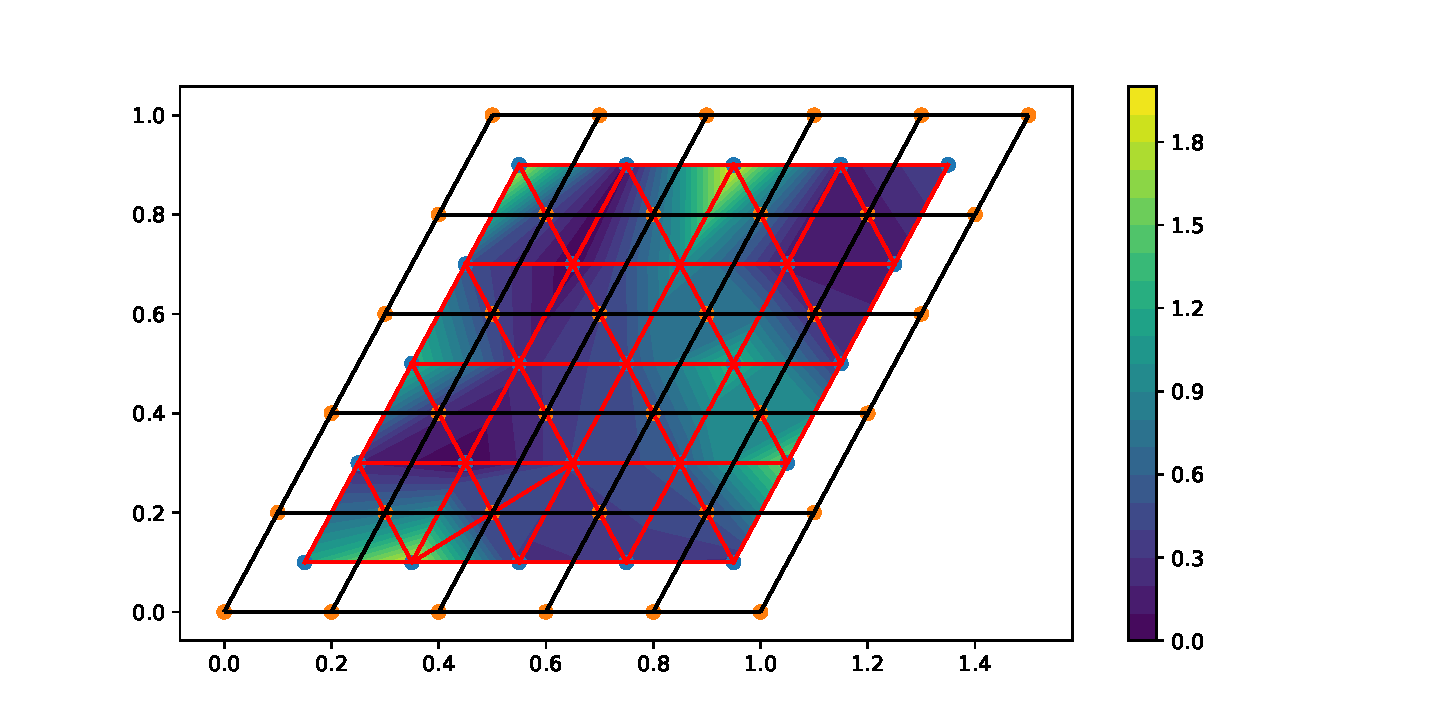
\includegraphics[width=1.1\textwidth]{L-triangles-heterogenous.pdf}
		\caption{L-triangles on a random permeability.}
		\label{fig:L-triangles-heterogeneous}
	\end{figure}


	\par 
	For homogenous media the L-method becomes easier to reason about. We continue with a useful theorem which we will use later:
	
	\begin{lemma}[Cao, Y., Helmig, R. and Wohlmuth, B.I. (2009),\cite{https://doi.org/10.1002/fld.1926}] \label{lemma:L_potential}
		Assume that the permeability $\bm{K}$ is homogenous on $\Omega$, then the flux through each half edge $e$, computed by the L-method, can be written as
		\begin{equation}\label{eq:L flux simplified}
			\tilde{q}_e = -\bm{K} \nabla u \cdot \bm{n}_e
		\end{equation}
		Where $\bm{n}_e$ is the scaled normal vector to the half edge $e$, having the same length as $e$. $u$ is a linear scalar field uniquely given by the potential values at the three cellcenters chosen by the L-method.
		\begin{figure}[H]
			\centering
			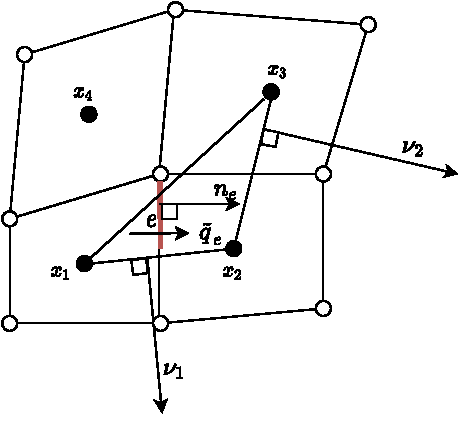
\includegraphics{Right choice linear potential.pdf}
			\caption{Simplified L-triangle, the original L-triangle i shown in figure \ref{fig:three sin x}. The vector $\nu_1$ is perpendicular to the edge between $x_1$ and $x_2$, with the same length as the edge it is perpendicular to. Same for $\nu_2$.}
			\label{fig:L-triangle-potential}
		\end{figure}
		Moreover, the gradient $\nabla u$, is given by:
		\begin{equation}\label{eq:L-potential}
			\nabla u = -\frac{1}{2F}[(u_1 - u_2)\nu_2 + (u_3 - u_2)\nu_1 ].
		\end{equation}
		Where $F$ is the the area of the simplified L-triangle with corners $x_1$, $x_2$ and $x_4$, see figure  \ref{fig:L-triangle-potential}. An expression like \eqref{eq:L-potential} can be obtained for the other choice of L-triangle as well.
	\end{lemma}
	\begin{figure}[H]
		\centering
		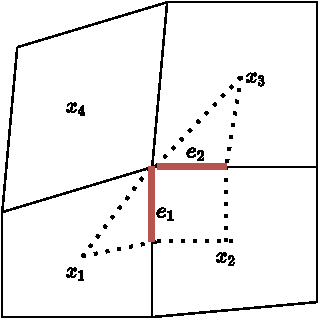
\includegraphics{right choice 2.pdf}	
		\caption{Original L-triangle with notations in proof.}
		\label{fig:original right choice}
	\end{figure}
	\begin{proof}
		It is enough to check that the jump $[\nabla u]$ is zero on $e_1$ and $e_2$ on the original L-triangle in figure \ref{fig:original right choice}. Let $\bm{t}_{e_1}$ and $\bm{n}_{e_1} $be the tangent and normal vector to $e_1$. Since we require potential continuity on each half edge, we get:
		\begin{equation}
			[\nabla u \cdot \bm{t}_{e_1}]=0.
		\end{equation}
		Using the fact that $\bm{K}$ is symmetric and homogenous, we obtain:
		\begin{equation}
			[\bm{K} \nabla u \cdot \bm{n}_{e_1}]=[\nabla u \cdot \bm{K}^T \bm{n}_{e_1}]=[\nabla u \cdot \bm{K}\bm{n}_{e_1}]=0.
		\end{equation}
		Where we used flux continuity across each half edge in the last equality. Since $\bm{K}$ is positive definite, we have that $\bm{K}\bm{n}_{e_1}$ and $\bm{t}_{e_1}$ are independent, thus $[\nabla u]=0$ on $e_1$. Same arguments holds for $e_2$. Hence $\nabla u$ is constant on the original L-triangle and the desired result follows.
	\end{proof}
	\begin{remark}
		The above lemma suggests that we can obtain the transmissibility coefficients without solving a system of equations for each half edge. This simplifies implementation, but it's only possible for homogenous media.
	\end{remark}
	\begin{remark}
		In the case of heterogeneous media, we do not easily get meaningful, physical interpretations of the transmissibility coefficients. Like the harmonic mean, as we did for TPFA. 
	\end{remark}
	\par 
	To conclude; the L-method is the most sophisticated method. It has the best monotonicity properties, it is consistent for non K orthogonal grids, but it requires more work for assembling the matrix. It is also more complicated to implement, especially for more dimensions.
	\section*{Time Discretization}	\addcontentsline{toc}{section}{Time Discretization}
		We start by considering the most famous parabolic equation, namely the heat equation. Let $u = u(x,t)$, given appropriate boundary and initial conditions, find $u$ such that:
	
	\begin{equation}\label{eq:heat equation}
		\begin{aligned}[c]
			\partial_t u - \nabla \cdot \pmb{K} \nabla u &= f \\
			u &= 0 \\
			\pmb{K}\nabla u &= g_N\\
			u &= u_0
		\end{aligned}
		\ \ \
		\begin{aligned}[c]
			x &\in \Omega  \\
			x &\in \partial \Gamma_D \\
			x &\in \partial \Gamma_N \\
			x &\in \Omega  
		\end{aligned}
		\ \ \
		\begin{aligned}
			t&\in (0,T] \\
			t&\in (0,T] \\
			t&\in (0,T] \\
			t&=0
		\end{aligned}
	\end{equation}
	The well-posedness of \eqref{eq:heat equation} is discussed in chapter seven of \cite{evans10}, it requires a more detailed discussion of Sobolev spaces and Bochner spaces, ie. spaces containing functions from the real numbers to some Sobolev space.\par
	We expect low regularity in time, so there is not much gained by using a higher order discretization in time. The two choices we have left is the forward euler(explicit) and the backward euler(implicit). The obvious choice is backward euler, as it is stable for long timesteps. This can be understood intuitively by considering the parabolic nature of the equation, the signals spread through the domain instantaneously. A careful analysis of time discretizations of parabolic equations is done in (\cite{Knabner}, chapter 7).  Here it is shown that explicit schemes only are stable for time-step proportional to the square of the space step, whereas fully implicit schemes are stable for all time-steps. \par  Let $\left \{ t_n \right \}_n$ be a sequence of $N+1$ evenly spaced numbers from $0$ to $T$ and let $\tau = \frac{T}{N}$ be the time-step. Then we state the semi-discrete version of \eqref{eq:heat equation} by exchanging the time derivative by a difference quotient $(\partial_t u)^n = \frac{u^n-u^{n-1}}{\tau}$. Note that this difference quotient is implicit because $u^n$ is not explicitly given by terms of the previous time-step. We end up with: Given $u^{n-1}$ and $f^n$, find $u^n$ such that
	\begin{equation}\label{eq:semidiscrete heat}
		\begin{aligned}[c]
			u^n - \tau \nabla \cdot \pmb{K} \nabla u^n &= \tau f^n+u^{n-1}\\
			u^n &= 0 \\
			\pmb{K}\nabla u &= g_N\\
			u^0 &= u_0
		\end{aligned}
		\ \ \
		\begin{aligned}[c]
			x &\in \Omega  \\
			x &\in \partial \Gamma_D \\
			x &\in \partial \Gamma_N \\
			x &\in \Omega .
		\end{aligned}
	\end{equation}
	Now we have an elliptic problem \eqref{eq:semidiscrete heat} for each time-step. This has almost the same structure as the elliptic model problem \eqref{eq:poisson} we solved in the previous chapters, the difference being that we have a $u^n$ term.
	\subsection*{Finite element approach}
	We are now ready to fit this problem into our finite element framework from chapter 2.
	The variational formulation of \eqref{eq:semidiscrete heat} is achieved as before by multiplying by test functions in $H^1_0(\Omega)$: Given $u^{n-1}$ in $V$, $f^n$ in the dual of $V$, find $u^n$ in $V$ such that
	\begin{equation}
			\left \langle  u^n, v\right \rangle_0 + \tau \left \langle  \pmb{K} \nabla u^n, \nabla v \right \rangle_0 =\tau \left \langle f^n,v\right \rangle_0 + \left \langle u^{n-1},v \right \rangle_0
	\end{equation}
	for all $v$ in $V$.
	If we swap $V$ with  a finite dimensional subspace $V_h$, and write $u_h^n = \sum_{i = 1}^d \hat{u}_i^n \phi_i $, as in the Galerkin FEM section, we end up with the system.
	\begin{equation}\label{eq:heat fem disc}
		\begin{aligned}
			\text{find }\hat{\bm{u}}^n&\in \mathbb{R}^d \text{ such that }\\
			\pmb{B}\hat{\bm{u}}^n+\tau\pmb{A}\hat{\bm{u}}^n &=\tau \pmb{f}^n +  \pmb{B}\hat{\bm{u}}^{n-1}
		\end{aligned}
	\end{equation}
	Where the \emph{stiffness matrix}, $\pmb{A}$, is as before. The matrix $\pmb{B}$ is often called the \emph{mass matrix} and is defined as $\pmb{B}_{i,j} = \int_{\Omega} \phi_i \phi_jdx$.
	\subsection*{Finite volume approach}
	As before we divide our domain $\Omega$ into control volumes $\left \{ \Omega_i \right \}_i$. One could write the heat equation\eqref{eq:heat equation} in conservation form on each control volume
	\begin{equation}\label{eq:semidiscrete FVM}
		\partial_t\int_{\Omega_i}u \ dx -\int_{\partial \Omega_i} \pmb{K}\nabla u \cdot \hat{\pmb{n}}\ dx = \int_{\Omega_i} f \ dx,
	\end{equation}
	and discretize the first term with backward Euler. Or one could make sure the semi-discrete heat equation \eqref{eq:heat equation} holds for each control volume and use the divergence theorem. Both ways, we end up with
	\begin{equation}
		\int_{\Omega_i} u^n \ dx - \tau\int_{\partial \Omega_i} \pmb{K}\nabla u^n \cdot \hat{\pmb{n}}\ dx = \tau \int_{\Omega_i} f^n \ dx + \int_{\Omega_i} u^{n-1} \ dx.
	\end{equation}
	As in the previous section we end up with a system of equations, where superscript $V$ is just to distinct between FVM and FEM.
	\begin{equation}\label{eq:heat fvm disc}
		(\pmb{B}^V + \tau \pmb{A}^V)\pmb{u}^n = \tau \pmb{f}^n + \pmb{B}^V\pmb{u}^{n-1}
	\end{equation}
	The matrix $\pmb{A}^V$ is as in chapter 3, with the fluxes through the edges of cell $i$ described by the $j$th row of $\pmb{A}^V$. The matrix $\pmb{B}^V$ is diagonal with the entry $i$ being the volumes of the volume of cell $i$.
	
	If $\pmb{A}= \pmb{A}^V$, ie. that the discretization of the constitutive law is the same for both finite volume and finite element method. As we will see later, this is the challenging part.	
	\section*{Linearization}
Now we have seen that the heat equation leads to a sequence of linear systems. In the same way, we expect that our non-linear Richards' equation \eqref{eq:richards} leads to a system of non-linear equations. We start by discussing this in a general setting
\begin{equation}\label{eq:non-linear-problem}
	\text{find }x\in U \text{ such that }\pmb{f}(\pmb{x})=\pmb{0} \\ \text{ where } f:U\subset\mathbb{R}^n\rightarrow\mathbb{R}^n
\end{equation}
The solution in \eqref{eq:non-linear-problem} is called a \emph{root}, it is almost always found using an iterative method.\par 
A common iterative scheme to solve \eqref{eq:non-linear-problem} is the \emph{Newton method}, let $D\pmb{f}(\pmb{x}_{j-1})^{-1}:\mathbb{R}^n\rightarrow\mathbb{R}^n$ be the Jacobian of $\pmb{f}(\pmb{x}_{j-1})$.
\begin{equation}
	\pmb{x}_j = \pmb{x}_{j-1} -D\pmb{f}(\pmb{x}_{j-1})^{-1}\pmb{f}(\pmb{x}_{j-1})
\end{equation}
In one dimension a convergence proof i easily obtained by techniques from calculus, the following theorem is found in  slightly more detail in (Cheney\cite{Cheney}, chapter 3):
\begin{theorem}
	Let $f''<2$ with $f(\overline{x})=0$ and $f'(x)> \delta \ \forall x \in B_{\epsilon}(\overline{x})$, then the Newton method is locally quadratic convergent:  For $x_0\in B_{\epsilon}(\overline{x})$ we have
	\begin{equation}
		| x_{j+1}-\overline{x}| \leq \frac{1}{\delta}|x_j - \overline{x}|^2< |x_j-\overline{x}|
	\end{equation}
\end{theorem}
\begin{proof}
	Define $e_n=x_n-\overline{x}$. Then we have by Taylor expansion
	\begin{equation}\label{eq:newton_taylor}
		0 = f(\overline{x})=f(x_j-e_j) = f(x_j)-f'(x_j)e_j + \frac{f''(\psi)e_j^2}{2}
	\end{equation}
	For some $\psi$ between $x_j$ and $\overline{x}$. Further we get by definition of the newton method
	\begin{equation}
		\begin{aligned}
			e_{j+1} = x_{j+1}-\overline{x} &= x_n-\frac{f(x_j)}{f'(x_j)}-\overline{x}\\
			&=e_j - \frac{f(x_j)}{f'(x_j)}\\ &= \frac{e_j f'(x_j)-f(x_j)}{f'(x_j)}
		\end{aligned}
	\end{equation}
	By the Taylor expansion around $x_j$, \eqref{eq:newton_taylor}, we get
	\begin{equation}
		e_{j+1} = \frac{e_j^2f''(\psi)}{2f'(x_j)}
	\end{equation}
	The assumptions on $f'$ and  $f''$ combined with $|e_0|<\delta$ give us the estimate
	\begin{equation}
		| e_{1} | \leq \frac{2}{2\delta}|e_0|^2<|e_0|
	\end{equation}
	By the same reasoning we get convergence
	\begin{equation}
		|e_{j+1}|<|e_j|
	\end{equation}
	And the quadratic convergence
	\begin{equation}
		| e_{j+1} | \leq \frac{1}{\delta}|e_j|^2
	\end{equation}
\end{proof}
For a similar result in more dimensions see (Knabner \cite{Knabner}, chapter 8). One apparent drawback of this method is that it's only locally convergent, ie. one needs to start the iteration in a neighbourhood of the root where the Jacobian is well defined. In practice one often solves the system
\begin{equation}
	D\pmb{f}(\pmb{x}_{j-1})\pmb{\delta}_{j} = -\pmb{f}(\pmb{x}_{j-1})
\end{equation}
And then update the current iterate with $\pmb{x}_j = \pmb{x}_{j-1} + \pmb{\delta}_{j}$. One often end end up with a situation where the matrix $D\pmb{f}(\pmb{x}_{j-1})$ needs to be computed and assembled for every iteration. This may be computationally expensive. So Newtons method may be slow despite it's quadratic convergence, if it even converges.\par 
A simpler approach is to swap the Jacobian with a diagonal matrix $L\pmb{I}$ such that 
\begin{equation}\label{eq:L-scheme}
	L\pmb{\delta}_j = - \pmb{f}(\pmb{x}_{j-1})
\end{equation}
This is called the \emph{L-scheme}, and will be method we will use for linearization in this thesis. In one dimension it is easy to prove convergence:

\begin{theorem}
	Let $f\in C(\mathbb{R})$ and $L>\sup_{x\in\mathbb{R}}f'(x)$, then the L-scheme converges linearly for all $x_0\in \mathbb{R}$.
\end{theorem}
\begin{proof}
	Define $e_j = e_j-\overline{x}$, then we get
	\begin{equation}
		e_{j+1} = x_j-\frac{f(x_j)}{L}-\overline{x}=e_j-\frac{f(x_j)}{L}
	\end{equation}
	We use the same trick as before with the Taylor expansion around the root.
	\begin{equation}
		0 = f(\overline{x}) = f(x_j-e_j) = f(e_j)-f'(\psi)e_j\Rightarrow e_j = \frac{f(x_j)}{f'(\psi)}
	\end{equation}
	Using this and the assumption on $L$ we get the estimate
	\begin{equation}
		|e_{j+1}|=|e_j(1-\frac{f'(\psi)f(x_j)}{f(x_j)L})|\leq|e_j||1-\frac{f'(\psi)}{L}|<|e_j|
	\end{equation}
\end{proof}


\end{document}